% L11a student companion deck: composite contracts, their net present value and
% profit at expiration, the common credit structures (short puts and calls, credit
% spreads, short straddles and strangles, protected strangles and iron condors),
% and why we wait to expiration.
%
% October 29, 2026: class ran behind in L10b, so its composite contract frames
% (everything after the Akuna Capital profile) moved here unchanged, with new
% title, objectives, What You Need to Know, examples, and summary frames. The
% L10b deck keeps its copy. Figures are the light PDFs in ../figs, renamed from
% Fig-L10b-* (see ../figs/README.md).
%
% The frame order mirrors the lecture notebook. The disclaimer is slide 2, by
% instructor preference. Notation follows the lecture: composite contract
% \mathcal{C} with legs i, orientation \theta_i, copy number n_i, strike K_i, leg
% payoff V_i(K_i,S(T)), composite payoff \hat{V}_{\mathcal{C}}(S(T)), composite premium
% \mathcal{P}_{\mathcal{C}}, profit at expiration \hat{P}_{\mathcal{C}}(S(T)),
% discount factor \mathcal{D}^{-1}_{T,0}(g_y), accumulation factor
% \mathcal{D}_{T,0}(g_y) (always written in full), and breakevens S^{\ddagger},
% S^{\ddagger}_{\pm}.
\documentclass[aspectratio=169,11pt]{beamer}
\usepackage{vnslides}

\newcommand{\Cc}{\mathcal{C}}
\newcommand{\Q}{\mathbb{Q}}
\newcommand{\Dc}{\mathcal{D}}
\newcommand{\Pc}{\mathcal{P}}
\newcommand{\repo}{https://github.com/varnerlab/CHEME-5660-CourseRepository-Fall-2026/blob/main/lectures/week-11/L11a}

\title{\texorpdfstring{{\vnheavy L11a}}{L11a}: Composite Contracts and Their Probability of Profit}
\subtitle{CHEME 5660 Cornell University}
\author{Copyright Jeffrey Varner 2026. All Rights Reserved}

\begin{document}

\vntitlepage

\begin{frame}{Disclaimer and Risks}
  \vspace{0.6em}
  \textbf{\ink{Training only.}} This content is for training and informational
  purposes only. The teaching team does not make, give, or endorse any offer or
  solicitation to buy or sell securities or derivative products, or provide
  investment or trading advice or strategy.

  \vspace{1.1em}
  \textbf{\ink{Risk.}} Trading involves risk and is generally not recommended for
  those with limited resources, experience, or a low risk tolerance. Past
  performance does not guarantee future success.

  \vspace{1.1em}
  \textbf{\ink{Responsibility.}} You are responsible for your investment decisions
  based on your financial circumstances, objectives, risk tolerance, and
  liquidity needs.
\end{frame}

\begin{frame}{Objectives for Today}
  Today, we combine single contracts into composite contracts. What is a
  composite contract worth, and when does it make money?

  \vspace{0.5em}
  {\large\textbf{\ink{Today's concepts}}}
  \begin{itemize}\setlength{\itemsep}{0.4em}
    \item \hilite{The NPV and POP of a composite contract}: sums over its legs.
    \item \hilite{Common composite contracts}: outlook, breakevens, maximum profit
      and loss.
    \item \hilite{Closing before expiration}: why an early exit earns less.
  \end{itemize}
\end{frame}

\begin{frame}{What You Need to Know}
  \vspace{0.3em}
  {\large\textbf{\ink{Core concepts}}}
  \begin{itemize}\setlength{\itemsep}{0.4em}
    \item Profit at expiration: the legs' payoffs, weighted by $\theta_{i}n_{i}$,
      minus the composite premium grown to expiration. POP: the probability it is
      positive.
    \item Read a profit diagram: the outlook, the breakevens, the maximum profit
      (the credit grown to expiration), and the maximum loss.
    \item Closing early earns less, by roughly the extrinsic value left in the
      legs. Near expiration, a small move near a strike changes the profit by more.
  \end{itemize}

  \vspace{0.5em}
  {\large\textbf{\ink{For understanding}} \dimmed{(you won't reproduce these)}}
  \begin{itemize}\setlength{\itemsep}{0.3em}
    \item The NPV derivation and the formula tables for the eight composite
      contracts.
  \end{itemize}
\end{frame}

\begin{frame}{Lectures and Examples}
  \vspace{0.3em}
  {\normalsize\textbf{\ink{Lecture:}}\par\small
  \href{\repo/CHEME-5660-L11a-Lecture-CompositeContracts-Fall-2026.ipynb}{\dimmed{CHEME-5660-L11a-Lecture-CompositeContracts-Fall-2026.ipynb}}}

  \vspace{0.6em}
  {\normalsize\textbf{\ink{Example 1:}}\par\small
  \href{\repo/CHEME-5660-L11a-Example-Delta-VerticalSpread-Fall-2026.ipynb}{\dimmed{CHEME-5660-L11a-Example-Delta-VerticalSpread-Fall-2026.ipynb}}}

  \vspace{0.45em}
  {\normalsize\textbf{\ink{Example 2:}}\par\small
  \href{\repo/CHEME-5660-L11a-Example-Straddle-AMD-Earnings-Fall-2026.ipynb}{\dimmed{CHEME-5660-L11a-Example-Straddle-AMD-Earnings-Fall-2026.ipynb}}}
\end{frame}

% ========== Composite Contracts
\begin{frame}{Composite Contracts}
  A composite contract $\Cc$ combines long and short puts and calls on one
  underlying asset with one expiration date $T$. Its payoff per share at
  expiration is:
  \begin{equation*}
    \hat{V}_{\Cc}(S(T)) = \underbrace{\sum_{i\in\Cc}\theta_{i}\;n_{i}\;\overbrace{V_{i}(K_{i},S(T))}^{\textstyle\text{payoff of leg } i}}_{\textstyle\text{sum of all legs}}
  \end{equation*}
  Here $S(T)$ is the share price at expiration, $K_{i}$ the strike price of leg
  $i$, $V_{i}$ its payoff, $(S(T)-K_{i})^{+}$ for a call or $(K_{i}-S(T))^{+}$ for
  a put, $n_{i}$ its number of contracts, and $\theta_{i}=-1$ if short or $1$ if
  long.
\end{frame}

\begin{frame}{The Net Present Value of a Composite Contract}
  A composite contract is a sum of legs, so its NPV is the sum of the legs'
  NPVs, weighted by $\theta_{i}n_{i}$:
  \begin{align*}
    \operatorname{NPV}_{0}(\Cc) &= \sum_{i\in\Cc}\theta_{i}\,n_{i}\underbrace{\Bigl(-\Pc_{i}+\overbrace{\Dc^{-1}_{T,0}(g_{y})\cdot V_{i}(K_{i},S(T))}^{\textstyle\text{discounted payoff}}\Bigr)}_{\textstyle\text{NPV of buying leg } i} && \text{weighted leg NPVs}\\
    &= -\underbrace{\sum_{i\in\Cc}\theta_{i}\,n_{i}\,\Pc_{i}}_{\textstyle=\,\Pc_{\Cc}}+\Dc^{-1}_{T,0}(g_{y})\cdot\underbrace{\sum_{i\in\Cc}\theta_{i}\,n_{i}\,V_{i}(K_{i},S(T))}_{\textstyle=\,\hat{V}_{\Cc}(S(T))} && \text{split the sum}\\
    &= -\Pc_{\Cc}+\Dc^{-1}_{T,0}(g_{y})\cdot\hat{V}_{\Cc}(S(T))
  \end{align*}
  where $\Pc_{i}$ is the premium of leg $i$ (USD/share), positive whether we buy
  or sell it ($\theta_{i}$ sets the direction), $\Pc_{\Cc}$ is the
  \hilite{composite premium}, and $\hat{V}_{\Cc}(S(T))$ is the
  \hilite{composite payoff}.
\end{frame}

\begin{frame}{Profit at Expiration}
  Factoring out $\Dc^{-1}_{T,0}(g_{y})$ writes the NPV as a profit at expiration
  discounted to today:
  \begin{align*}
    \operatorname{NPV}_{0}(\Cc) &= \Dc^{-1}_{T,0}(g_{y})\cdot\underbrace{\Bigl(\hat{V}_{\Cc}(S(T))-\Dc_{T,0}(g_{y})\cdot\Pc_{\Cc}\Bigr)}_{\textstyle=\,\hat{P}_{\Cc}(S(T))} && \text{factor out }\Dc^{-1}_{T,0}(g_{y})\\
    &= \Dc^{-1}_{T,0}(g_{y})\cdot\underbrace{\hat{P}_{\Cc}(S(T))}_{\makebox[0pt]{profit at expiration}}
  \end{align*}
  where $\Dc_{T,0}(g_{y})=e^{g_{y}T}$ is the accumulation factor, and:
  \begin{equation*}
    \boxed{\hat{P}_{\Cc}(S(T)) = \hat{V}_{\Cc}(S(T)) - \Dc_{T,0}(g_{y})\cdot\Pc_{\Cc}}
  \end{equation*}
  is the \hilite{profit at expiration} (USD/share).
\end{frame}

\begin{frame}{Debit or Credit}
  Because $\theta_{i}=1$ for a long leg and $\theta_{i}=-1$ for a short leg, the
  composite premium splits into the premium we pay and the premium we collect:
  \begin{equation*}
    \Pc_{\Cc}=\underbrace{\sum_{\text{long legs}}n_{i}\,\Pc_{i}}_{\textstyle\text{premium we pay}}-\underbrace{\sum_{\text{short legs}}n_{i}\,\Pc_{i}}_{\textstyle\text{premium we collect}}
  \end{equation*}
  If we pay more than we collect, $\Pc_{\Cc}>0$: a \hilite{debit}. If we collect
  more than we pay, $\Pc_{\Cc}<0$: the contract has a negative price to a buyer,
  so we are paid to open it, a \hilite{credit} of $-\Pc_{\Cc}$ USD/share. For
  example, selling one put with premium $\Pc_{p}$ gives $\Pc_{\Cc}=-\Pc_{p}$, a
  credit of $\Pc_{p}$.
\end{frame}

\begin{frame}{Probability of Profit and Probability of Exercise}
  The NPV and the profit at expiration have the same sign, so with $\mathbb{P}$
  our belief, the \hilite{probability of profit} is:
  \begin{equation*}
    \boxed{\text{POP}_{\Cc} = \mathbb{P}\Bigl(\operatorname{NPV}_{0}(\Cc)>0\Bigr) = \mathbb{P}\Bigl(\hat{P}_{\Cc}(S(T))>0\Bigr)}
  \end{equation*}
  Each leg has its own \hilite{probability of exercise}:
  \begin{equation*}
    \text{POE}_{i} = \begin{cases}
      \mathbb{P}\left(S(T)>K_{i}+0.01\right) & \text{if leg } i \text{ is a call}\\
      \mathbb{P}\left(S(T)<K_{i}-0.01\right) & \text{if leg } i \text{ is a put}
    \end{cases}
  \end{equation*}
\end{frame}

% ========== Common Composite Credit Contracts
\begin{frame}{Composite Credit Contracts: Outlook}
  The eight structures, by side:\par
  {\centering\footnotesize\setlength{\tabcolsep}{4pt}
    \begin{tabular}{llll}
      \toprule
      Composite contract & Put side & Call side & Outlook \\
      \midrule
      Short put & short put at $K$ & none & neutral to bullish \\
      Short call & none & short call at $K$ & neutral to bearish \\
      Put credit spread & \begin{tabular}[c]{@{}l@{}}short put at $K_{2}$\\ long put at $K_{1}<K_{2}$\end{tabular} & none & neutral to bullish \\
      Call credit spread & none & \begin{tabular}[c]{@{}l@{}}short call at $K_{1}$\\ long call at $K_{2}>K_{1}$\end{tabular} & neutral to bearish \\
      Short straddle & short put at $K$ & short call at $K$ & neutral \\
      Short strangle & short put at $K_{1}$ & short call at $K_{2}>K_{1}$ & neutral \\
      Protected strangle & short put at $K_{1}$ & \begin{tabular}[c]{@{}l@{}}short call at $K_{2}$\\ long call at $K_{3}>K_{2}$\end{tabular} & neutral, leaning bullish \\
      Iron condor & \begin{tabular}[c]{@{}l@{}}short put at $K_{2}$\\ long put at $K_{1}<K_{2}$\end{tabular} & \begin{tabular}[c]{@{}l@{}}short call at $K_{3}$\\ long call at $K_{4}>K_{3}$\end{tabular} & neutral \\
      \bottomrule
    \end{tabular}\par}
  \vspace{0.2em}
  {\small Strikes are numbered low to high, $\Pc_{i}$ is the premium of the leg at
  $K_{i}$. Figures: payoff (blue), profit (black), and $S(0)$, the share price at entry.}
\end{frame}

\begin{frame}{Composite Credit Contracts: Three Steps}
  Each row of the tables follows from the profit at expiration expression in three steps:
  \begin{enumerate}\setlength{\itemsep}{0.6em}
    \item Compute the composite premium $\Pc_{\Cc}$, with a minus sign for each
      short leg. If $\Pc_{\Cc}<0$, the contract opens for a credit of $-\Pc_{\Cc}$
      (a positive term in the profit at expiration).
    \item Write the profit on each interval between the strikes. There, each
      leg's payoff is zero or linear in $S(T)$, so the profit is a straight line.
    \item Evaluate the profit at the strikes, at $S(T)=0$, and as $S(T)$ grows,
      to find the maximum profit and maximum loss. Set the profit to zero where
      it slopes to find the breakevens, keeping each solution that lies in its
      interval.
  \end{enumerate}
  \vspace{0.4em}
  Maximum losses are listed as positive amounts (USD/share).
  \slidenote{Derivation:}{\href{\repo/CHEME-5660-L11a-Derivation-ProfitLossBreakeven-Fall-2026.ipynb}{\dimmed{CHEME-5660-L11a-Derivation-ProfitLossBreakeven-Fall-2026.ipynb}}}
\end{frame}

\begin{frame}{Buying Shares}
  Before combining options, let's look at the simplest position: buying one
  share at $S(0)$ and holding it to expiration. Its profit at expiration is the
  share price at expiration minus the purchase price grown to expiration:
  \begin{equation*}
    \hat{P}(S(T)) = S(T)-\Dc_{T,0}(g_{y})\cdot S(0)
  \end{equation*}
  The profit has no upper limit, but if the share price falls to zero, we lose
  the whole purchase price grown to expiration.
\end{frame}

\begin{frame}{Short Puts and Short Calls}
  Selling one put, a
  \href{https://www.fidelity.com/learning-center/investment-products/options/options-strategy-guide/shortput-uncovered}{\hilite{short put}},
  or one call, a
  \href{https://www.fidelity.com/learning-center/investment-products/options/options-strategy-guide/shortcall-uncovered}{\hilite{short call}},
  is the building block of every structure below:
  \begin{center}
    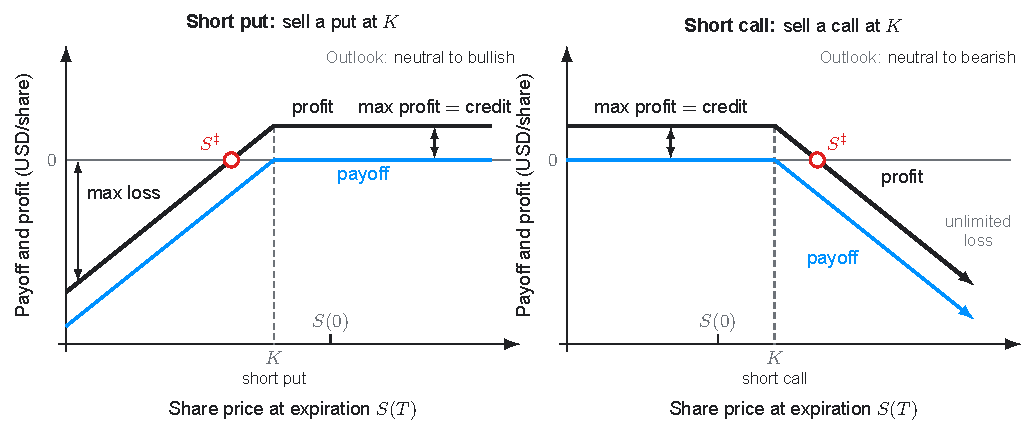
\includegraphics[width=\textwidth,height=0.58\textheight,keepaspectratio]{../figs/Fig-L11a-Short-Put-Call.pdf}
  \end{center}
  Each keeps the whole premium if it expires out of the money.
\end{frame}

\begin{frame}{Short Puts and Short Calls: Profit at Expiration}
  With premiums $\Pc_{p}$ (put) and $\Pc_{c}$ (call) at strike $K$, the profits
  at expiration, and the breakevens $S^{\ddagger}$, are:
  \begin{align*}
    \hat{P}_{\Cc}(S(T)) &= \Dc_{T,0}(g_{y})\cdot\Pc_{p}-(K-S(T))^{+} && \text{short put}\\
    \hat{P}_{\Cc}(S(T)) &= \Dc_{T,0}(g_{y})\cdot\Pc_{c}-(S(T)-K)^{+} && \text{short call}
  \end{align*}
  \begin{center}\small
    \begin{tabular}{lll}
      \toprule
      & Short put & Short call \\
      \midrule
      Maximum profit & $\Dc_{T,0}(g_{y})\cdot\Pc_{p}$ for $S(T)\geq K$ & $\Dc_{T,0}(g_{y})\cdot\Pc_{c}$ for $S(T)\leq K$ \\
      Breakeven & $S^{\ddagger}=K-\Dc_{T,0}(g_{y})\cdot\Pc_{p}$ & $S^{\ddagger}=K+\Dc_{T,0}(g_{y})\cdot\Pc_{c}$ \\
      Maximum loss & $K-\Dc_{T,0}(g_{y})\cdot\Pc_{p}$ at $S(T)=0$ & unlimited \\
      \bottomrule
    \end{tabular}
  \end{center}
  The short put's loss is bounded ($S(T)\geq0$); the short call's is not.
\end{frame}

\begin{frame}{Short Put Compared with One Share}
  Next to one share bought at $S(0)$, the short put has:
  \begin{center}\small
    \begin{tabular}{lll}
      \toprule
      & Short put & One share \\
      \midrule
      Maximum profit & $\Dc_{T,0}(g_{y})\cdot\Pc_{p}$ for $S(T)\geq K$ & unlimited \\
      Breakeven & $S^{\ddagger}=K-\Dc_{T,0}(g_{y})\cdot\Pc_{p}$ & $S^{\ddagger}=\Dc_{T,0}(g_{y})\cdot S(0)$ \\
      Maximum loss & $K-\Dc_{T,0}(g_{y})\cdot\Pc_{p}$ at $S(T)=0$ & $\Dc_{T,0}(g_{y})\cdot S(0)$ at $S(T)=0$ \\
      \bottomrule
    \end{tabular}
  \end{center}
  With $S(0)=K$, the short put breaks even lower and has a smaller maximum loss,
  but its profit stops at the credit grown to expiration. All entries are per
  share: one contract covers 100 shares, so multiply by 100 to compare one
  contract with 100 shares.
\end{frame}

\begin{frame}{Credit Spreads}
  A \hilite{credit spread} sells the contract closer to the share price and buys
  one farther away, same type and expiration (a
  \href{https://www.fidelity.com/learning-center/investment-products/options/options-strategy-guide/bull-put-spread}{\hilite{bull put}}
  or
  \href{https://www.fidelity.com/learning-center/investment-products/options/options-strategy-guide/bear-call-spread}{\hilite{bear call}}
  spread):
  \begin{center}
    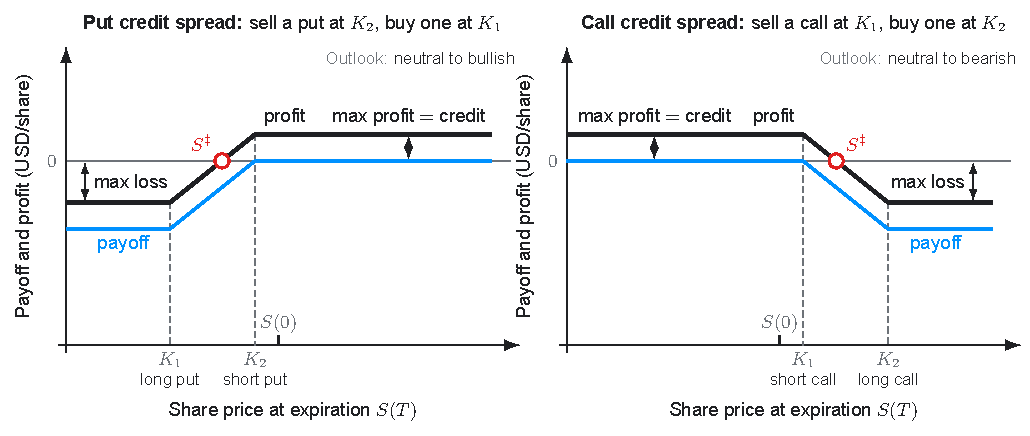
\includegraphics[width=\textwidth,height=0.55\textheight,keepaspectratio]{../figs/Fig-L11a-Credit-Spreads.pdf}
  \end{center}
  The short leg collects the credit; the long leg caps the loss.
\end{frame}

\begin{frame}{Put Credit Spread}
  A long put at $K_{1}$ and a short put at $K_{2}$: the credit grown to
  expiration, minus and plus the leg payoffs:
  \begin{equation*}
    \hat{P}_{\Cc}(S(T)) = \Dc_{T,0}(g_{y})\cdot(\Pc_{2}-\Pc_{1})-(K_{2}-S(T))^{+}+(K_{1}-S(T))^{+}
  \end{equation*}
  \begin{center}\small
    \begin{tabular}{ll}
      \toprule
      Maximum profit & $\Dc_{T,0}(g_{y})\cdot(\Pc_{2}-\Pc_{1})$ for $S(T)\geq K_{2}$ \\
      Breakeven & $S^{\ddagger}=K_{2}-\Dc_{T,0}(g_{y})\cdot(\Pc_{2}-\Pc_{1})$ \\
      Maximum loss & $(K_{2}-K_{1})-\Dc_{T,0}(g_{y})\cdot(\Pc_{2}-\Pc_{1})$ for $S(T)\leq K_{1}$ \\
      \bottomrule
    \end{tabular}
  \end{center}
  \slidenote{Example 1:}{\href{\repo/CHEME-5660-L11a-Example-Delta-VerticalSpread-Fall-2026.ipynb}{\dimmed{CHEME-5660-L11a-Example-Delta-VerticalSpread-Fall-2026.ipynb}}}
\end{frame}

\begin{frame}{Call Credit Spread}
  A short call at $K_{1}$ and a long call at $K_{2}$ give the profit at
  expiration:
  \begin{equation*}
    \hat{P}_{\Cc}(S(T)) = \Dc_{T,0}(g_{y})\cdot(\Pc_{1}-\Pc_{2})-(S(T)-K_{1})^{+}+(S(T)-K_{2})^{+}
  \end{equation*}
  \begin{center}\small
    \begin{tabular}{ll}
      \toprule
      Maximum profit & $\Dc_{T,0}(g_{y})\cdot(\Pc_{1}-\Pc_{2})$ for $S(T)\leq K_{1}$ \\
      Breakeven & $S^{\ddagger}=K_{1}+\Dc_{T,0}(g_{y})\cdot(\Pc_{1}-\Pc_{2})$ \\
      Maximum loss & $(K_{2}-K_{1})-\Dc_{T,0}(g_{y})\cdot(\Pc_{1}-\Pc_{2})$ for $S(T)\geq K_{2}$ \\
      \bottomrule
    \end{tabular}
  \end{center}
  Beyond the long strike, the long leg gains what the short leg loses, so the
  loss stops at the strike width minus the credit.
\end{frame}

\begin{frame}{Short Straddles and Strangles}
  A \href{https://www.fidelity.com/learning-center/investment-products/options/options-strategy-guide/short-straddle}{\hilite{straddle}}:
  a put and a call at one strike $K$. A
  \href{https://www.fidelity.com/learning-center/investment-products/options/options-strategy-guide/short-strangle}{\hilite{strangle}}: a
  put at $K_{1}$ below a call at $K_{2}$. Same expiration:
  \begin{center}
    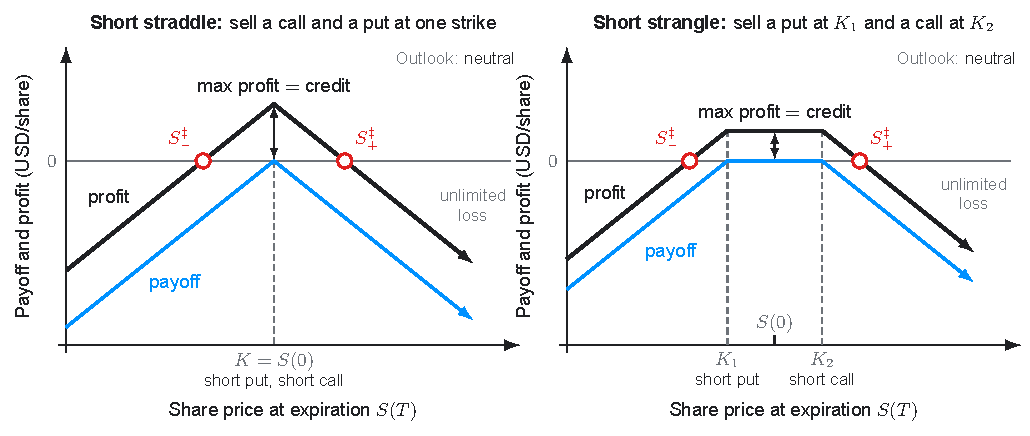
\includegraphics[width=\textwidth,height=0.55\textheight,keepaspectratio]{../figs/Fig-L11a-Straddle-Strangle.pdf}
  \end{center}
  Sold, each profits only between its breakevens:
  $\text{POP}=\mathbb{P}(S^{\ddagger}_{-}<S(T)<S^{\ddagger}_{+})$.
\end{frame}

\begin{frame}{Short Straddle}
  Selling a put and a call at the strike $K$ gives the profit at expiration:
  \begin{equation*}
    \hat{P}_{\Cc}(S(T)) = \Dc_{T,0}(g_{y})\cdot(\Pc_{p}+\Pc_{c})-(K-S(T))^{+}-(S(T)-K)^{+}
  \end{equation*}
  \begin{center}\small
    \begin{tabular}{ll}
      \toprule
      Maximum profit & $\Dc_{T,0}(g_{y})\cdot(\Pc_{p}+\Pc_{c})$ at $S(T)=K$ \\
      Lower breakeven & $S^{\ddagger}_{-}=K-\Dc_{T,0}(g_{y})\cdot(\Pc_{p}+\Pc_{c})$ \\
      Maximum loss below $S^{\ddagger}_{-}$ & $K-\Dc_{T,0}(g_{y})\cdot(\Pc_{p}+\Pc_{c})$ at $S(T)=0$ \\
      Upper breakeven & $S^{\ddagger}_{+}=K+\Dc_{T,0}(g_{y})\cdot(\Pc_{p}+\Pc_{c})$ \\
      Maximum loss above $S^{\ddagger}_{+}$ & unlimited \\
      \bottomrule
    \end{tabular}
  \end{center}
  The straddle collects more credit, but the strangle keeps its credit over a
  wider range of share prices.
\end{frame}

\begin{frame}{Short Strangle}
  Selling a put at $K_{1}$ and a call at $K_{2}$ gives the profit at expiration:
  \begin{equation*}
    \hat{P}_{\Cc}(S(T)) = \Dc_{T,0}(g_{y})\cdot(\Pc_{1}+\Pc_{2})-(K_{1}-S(T))^{+}-(S(T)-K_{2})^{+}
  \end{equation*}
  \begin{center}\small
    \begin{tabular}{ll}
      \toprule
      Maximum profit & $\Dc_{T,0}(g_{y})\cdot(\Pc_{1}+\Pc_{2})$ for $K_{1}\leq S(T)\leq K_{2}$ \\
      Lower breakeven & $S^{\ddagger}_{-}=K_{1}-\Dc_{T,0}(g_{y})\cdot(\Pc_{1}+\Pc_{2})$ \\
      Maximum loss below $S^{\ddagger}_{-}$ & $K_{1}-\Dc_{T,0}(g_{y})\cdot(\Pc_{1}+\Pc_{2})$ at $S(T)=0$ \\
      Upper breakeven & $S^{\ddagger}_{+}=K_{2}+\Dc_{T,0}(g_{y})\cdot(\Pc_{1}+\Pc_{2})$ \\
      Maximum loss above $S^{\ddagger}_{+}$ & unlimited \\
      \bottomrule
    \end{tabular}
  \end{center}
  \slidenote{Example 2:}{\href{\repo/CHEME-5660-L11a-Example-Straddle-AMD-Earnings-Fall-2026.ipynb}{\dimmed{CHEME-5660-L11a-Example-Straddle-AMD-Earnings-Fall-2026.ipynb}}}
\end{frame}

\begin{frame}{Protected Strangles and Iron Condors}
  A \hilite{protected strangle}
  (\href{https://www.tastylive.com/concepts-strategies/jade-lizard}{\hilite{jade lizard}})
  adds a long call at $K_{3}$ to a short strangle; an
  \href{https://www.fidelity.com/learning-center/investment-products/options/options-strategy-guide/short-iron-condor-spread}{\hilite{iron condor}}
  also adds a long put:
  \begin{center}
    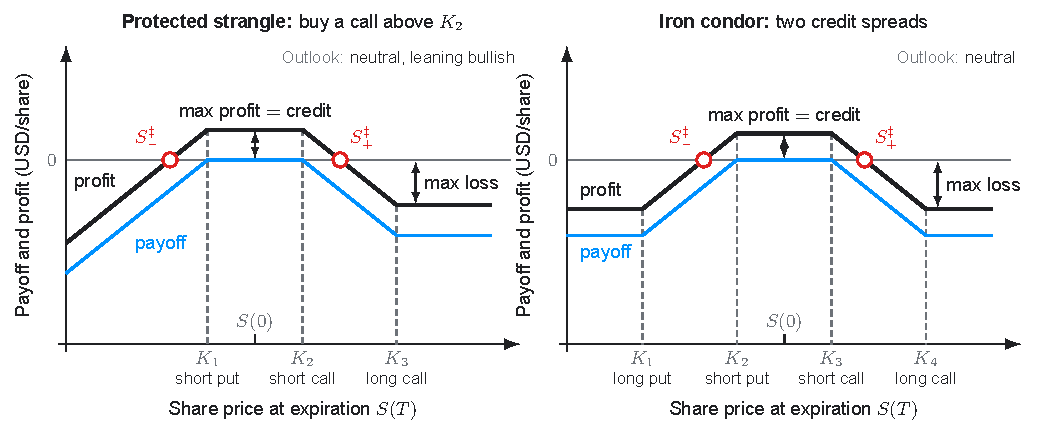
\includegraphics[width=\textwidth,height=0.58\textheight,keepaspectratio]{../figs/Fig-L11a-Protected-Condor.pdf}
  \end{center}
  Each long leg caps the loss on its side but lowers the credit.
\end{frame}

\begin{frame}{Protected Strangle}
  A short put at $K_{1}$, a short call at $K_{2}$, and a long call at $K_{3}$
  give the profit at expiration:
  \begin{align*}
    \hat{P}_{\Cc}(S(T)) &= \Dc_{T,0}(g_{y})\cdot(\Pc_{1}+\Pc_{2}-\Pc_{3}) && \text{protected strangle}\\
    &\qquad-(K_{1}-S(T))^{+}-(S(T)-K_{2})^{+}+(S(T)-K_{3})^{+}
  \end{align*}
  \begin{center}\footnotesize
    \begin{tabular}{ll}
      \toprule
      Maximum profit & $\Dc_{T,0}(g_{y})\cdot(\Pc_{1}+\Pc_{2}-\Pc_{3})$ for $K_{1}\leq S(T)\leq K_{2}$ \\
      Lower breakeven & $S^{\ddagger}_{-}=K_{1}-\Dc_{T,0}(g_{y})\cdot(\Pc_{1}+\Pc_{2}-\Pc_{3})$ \\
      Maximum loss below $S^{\ddagger}_{-}$ & $K_{1}-\Dc_{T,0}(g_{y})\cdot(\Pc_{1}+\Pc_{2}-\Pc_{3})$ at $S(T)=0$ \\
      Upper breakeven & $S^{\ddagger}_{+}=K_{2}+\Dc_{T,0}(g_{y})\cdot(\Pc_{1}+\Pc_{2}-\Pc_{3})$${}^{a}$ \\
      Maximum loss above $S^{\ddagger}_{+}$ & $(K_{3}-K_{2})-\Dc_{T,0}(g_{y})\cdot(\Pc_{1}+\Pc_{2}-\Pc_{3})$ for $S(T)\geq K_{3}$${}^{b}$ \\
      \bottomrule
    \end{tabular}
  \end{center}
  {\footnotesize ${}^{a}$If $\Dc_{T,0}(g_{y})\cdot(\Pc_{1}+\Pc_{2}-\Pc_{3})\leq K_{3}-K_{2}$; otherwise none. ${}^{b}$If $\Dc_{T,0}(g_{y})\cdot(\Pc_{1}+\Pc_{2}-\Pc_{3})<K_{3}-K_{2}$; otherwise none.\par}
  \vspace{0.3em}
  If the credit grown to expiration is at least $K_{3}-K_{2}$, the call side
  cannot lose.
\end{frame}

\begin{frame}{Iron Condor}
  A long put at $K_{1}$, a short put at $K_{2}$, a short call at $K_{3}$, and a
  long call at $K_{4}$ give the profit at expiration:
  \begin{align*}
    \hat{P}_{\Cc}(S(T)) &= \Dc_{T,0}(g_{y})\cdot(\Pc_{2}+\Pc_{3}-\Pc_{1}-\Pc_{4})\\
    &\qquad+(K_{1}-S(T))^{+}-(K_{2}-S(T))^{+}-(S(T)-K_{3})^{+}+(S(T)-K_{4})^{+}
  \end{align*}
  \begin{center}\footnotesize
    \begin{tabular}{ll}
      \toprule
      Maximum profit & $\Dc_{T,0}(g_{y})\cdot(\Pc_{2}+\Pc_{3}-\Pc_{1}-\Pc_{4})$ for $K_{2}\leq S(T)\leq K_{3}$ \\
      Lower breakeven & $S^{\ddagger}_{-}=K_{2}-\Dc_{T,0}(g_{y})\cdot(\Pc_{2}+\Pc_{3}-\Pc_{1}-\Pc_{4})$ \\
      Maximum loss below $S^{\ddagger}_{-}$ & $(K_{2}-K_{1})-\Dc_{T,0}(g_{y})\cdot(\Pc_{2}+\Pc_{3}-\Pc_{1}-\Pc_{4})$ for $S(T)\leq K_{1}$ \\
      Upper breakeven & $S^{\ddagger}_{+}=K_{3}+\Dc_{T,0}(g_{y})\cdot(\Pc_{2}+\Pc_{3}-\Pc_{1}-\Pc_{4})$ \\
      Maximum loss above $S^{\ddagger}_{+}$ & $(K_{4}-K_{3})-\Dc_{T,0}(g_{y})\cdot(\Pc_{2}+\Pc_{3}-\Pc_{1}-\Pc_{4})$ for $S(T)\geq K_{4}$ \\
      \bottomrule
    \end{tabular}
  \end{center}
  At any share price at expiration, at most one side can lose, so the maximum
  loss is the wider strike width minus the credit.
\end{frame}

\begin{frame}{Why Wait to Expiration?}
  Our diagrams are drawn at expiration. Closing a short leg early means buying it back: intrinsic plus extrinsic value
  $E_{V}(t)$. A short strangle (put $K_{1}=90$, call $K_{2}=110$, $S(0)=100$
  USD/share, 30 days, CRR tree, $\sigma=0.40$, $g_{y}=4\%$):
  \begin{center}
    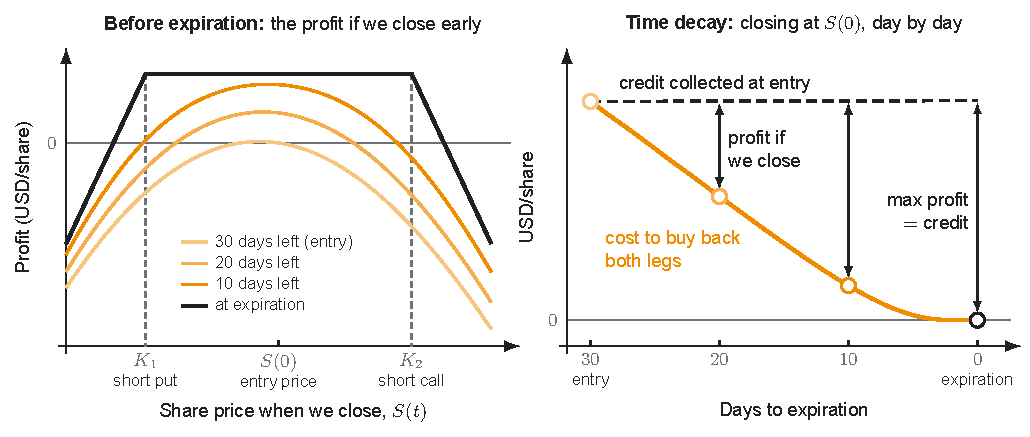
\includegraphics[width=\textwidth,height=0.55\textheight,keepaspectratio]{../figs/Fig-L11a-Strangle-Time-Decay.pdf}
  \end{center}
\end{frame}

\begin{frame}{Why Wait to Expiration? What Do We See?}
  \begin{itemize}\setlength{\itemsep}{0.6em}
    \item \hilite{Before expiration (left)}: the buyback price still includes
      extrinsic value, so earlier curves lie below the profit at expiration.
    \item \hilite{At the entry share price (right)}: both legs are out of the
      money, so closing at once costs exactly the credit and earns nothing.
    \item \hilite{Time decay}: as the extrinsic value decays, the profit if we
      close at $S(0)$ rises to the whole credit.
  \end{itemize}
  \vspace{0.4em}
  The diagrams show the most each contract can earn; an early exit earns less,
  by roughly the extrinsic value left in the legs.
\end{frame}

\begin{frame}{Summary}
  \vspace{0.3em}
  {\large\textbf{\ink{Key takeaways}}}
  \begin{itemize}\setlength{\itemsep}{0.4em}
    \item \hilite{The NPV of a composite contract is a sum over its legs}: the POP
      is the probability that the profit at expiration is positive.
    \item \hilite{Common composite contracts can be bullish, bearish, or neutral}:
      the profit diagram gives the outlook, breakevens, and maximum loss.
    \item \hilite{Closing before expiration earns less}: buying the legs back
      still pays for their extrinsic value.
  \end{itemize}
\end{frame}

\end{document}
